%%%%%%%%%%%%%%%%%%%%%%%%%%%%%%%%%%%55%%
\begin{frame} [plain]
    \frametitle{}
    \Background[1] 
    \begin{center}
    { {\huge 第十一讲、算符运动方程 }}
    \end{center}  
    \addtocounter{framenumber}{-1}   
\end{frame}
%%%%%%%%%%%%%%%%%%%%%%%%%%%%%%%%%%

%%%%%%%%%%%%%%%%%%%%%%%%%%%%%%%%%
\begin{frame}
        \frametitle{主要内容}
        \transfade
        \tableofcontents
        \addtocounter{framenumber}{-1} 
\end{frame}
%%%%%%%%%%%%%%%%%%%%%%%%%%%%%%%%%%


\section{前情回顾}

\begin{frame}
    \frametitle{前情回顾}
    \begin{itemize}
        \item 希尔伯特空间的态矢量描述体系状态
        \item 希尔伯特空间的算符给出体系的物理量
        \item 算符的本征函数系构成正交归一完全基
        \item 常见算符本征方程求解
        \item 算符对易关系及其物理含义 
    \end{itemize}   
\end{frame} 

\section{守恒量}

\begin{frame}
\includegraphics[width=0.6\textwidth]{figs/2021-12-17-21-25-13.png} \\
1918年 德国数学家 A. E. Noether : 从自然界的每一对称性可
得到一守恒律;反之,每一个守恒律均揭示蕴含其中的一种对称性。
\end{frame} 

\begin{frame} 
    \frametitle{守恒量定义}
    \begin{enumerate}
        \item  经典物理中的守恒量与对称条件\\
                守恒量:力学量的值不随时间变化\\
                \begin{itemize}
                    \item 机械能空间平移不变→动量守恒
                    \item 机械能空间转动不变→角动量守恒
                    \item 机械能时间平移不变→能量守恒
                \end{itemize}
        \item  量子力学中的守恒量\\
                守恒量:在任意态下力学量的平均值不随时间变化\\
                $$ \bar{F}(t)=(\Psi(t), F\Psi(t)) =c.  $$
                守恒量及守恒条件... 
    \end{enumerate}
\end{frame} 

\begin{frame} [allowframebreaks=]
    \frametitle{算符运动方程}    
        \begin{equation*}
            \begin{split} 
            \bar{F}(t)&=(\Psi(t), F(t)\Psi(t)) \\
            \frac{d\bar{F}}{dt}&=(\frac{\partial\Psi }{\partial t}, F\Psi) +(\Psi, \frac{\partial F }{\partial t}\Psi) +(\Psi, F\frac{\partial\Psi }{\partial t}) \\
            &= - \frac{1}{i\hbar} (H\Psi, F\Psi)+(\Psi, \frac{\partial F }{\partial t}\Psi) + \frac{1}{i\hbar} (\Psi, FH\Psi) \\
            &= - \frac{1}{i\hbar} (\Psi, HF\Psi)+(\Psi, \frac{\partial F }{\partial t}\Psi) + \frac{1}{i\hbar} (\Psi, FH\Psi) \\
            &= (\Psi, \frac{\partial F }{\partial t}\Psi)  +\frac{1}{i\hbar} (\Psi, [F,H]\Psi) \\
            &=\overline{(\frac{\partial F }{\partial t})}  +\frac{1}{i\hbar} \overline{[F,H]} \\
            \end{split}  
        \end{equation*}  
\end{frame} 

\begin{frame} [allowframebreaks=]
        \frametitle{力学量守恒条件} 
        由守恒量定义:   
        $$ \bar{F}(t)=(\Psi(t), F\Psi(t)) =c.  $$
        $$\frac{d\bar{F}}{dt}=\overline{(\frac{\partial F }{\partial t})}  +\frac{1}{i\hbar} \overline{[F,H]}=0$$
        得守恒量条件:
        $$\left\{\begin{aligned}
            &\frac{\partial F }{\partial t}=0\\
            &[F,H]=0 \\
        \end{aligned} \right. $$
\end{frame}

\begin{frame} 
    \frametitle{守恒量性质} 
    \begin{tcolorbox1}{性质1:}
        守恒量测量值概率分布不随时间改变
    \end{tcolorbox1}
    \alert{证明:} F是守恒量,则 $[F,H]=0$, 设F,H的共同本征函数系$\{\varphi_n\}$, 有:\\ 
    任意态$\Psi(t)$在$\{\varphi_n\}$展开,其展开系数为:
    $$C_n(t)=(\varphi_n, \Psi(t))$$
    展开系数的模方即为测量值为本征值$f_n$的概率,因此要证明:
    $$\frac{d}{dt} |C_n(t)|^2=0$$
\end{frame}

\begin{frame} [allowframebreaks=]
    $$\begin{aligned}
      \frac{d}{dt} |C_n(t)|^2 &= \frac{d}{dt} C_n^* C_n \\
      &=C_n \frac{d}{dt} C_n^*  +  C_n^*\frac{d}{dt}C_n \\
      &=[C_n^*[\frac{d}{dt} C_n]^*  +  [C_n^*\frac{d}{dt}C_n] \\
    \end{aligned}$$
    $$\begin{aligned}
      C_n^*\frac{d}{dt}C_n&= (\varphi_n, \Psi)^* \frac{d}{dt}(\varphi_n, \Psi) \\
      &= (\varphi_n, \Psi)^* (\varphi_n, \frac{d}{dt}\Psi) \\
      &= \frac{1}{i\hbar}(\varphi_n, \Psi)^* (\varphi_n, H\Psi) \\
      &= \frac{1}{i\hbar}(\varphi_n, \Psi)^* (H\varphi_n, \Psi) = \frac{E_n}{i\hbar}C_n ^* C_n 
    \end{aligned}$$
    $$\begin{aligned}
        \frac{d}{dt} |C_n(t)|^2 &= [C_n^*[\frac{d}{dt} C_n]^*  +  [C_n^*\frac{d}{dt}C_n] \\
        &= [\frac{E_n}{i\hbar}C_n ^* C_n ]^* + \frac{E_n}{i\hbar}C_n ^* C_n \\
        &= -\frac{E_n}{i\hbar}C_n ^* C_n ] + \frac{E_n}{i\hbar}C_n ^* C_n \\
        &=0
    \end{aligned}$$
      证毕!
    \begin{tcolorbox2}{结论:}
        无论体系本征态还是叠加态(任意态),守恒量的平均值及各测量值的概率分布都不随时间变化。         
    \end{tcolorbox2}
\end{frame}

\begin{frame} [allowframebreaks=]
    \frametitle{} 
    \begin{tcolorbox1}{性质2:}
        若体系有两个不对易守恒量,则一般存在简并能级
    \end{tcolorbox1}
    \alert{证明:} 设F、G都是体系的守恒量,则有 $[F,H]=0$, $[G,H]=0$, 设F,H的共同本征函数系$\{\varphi_n\}$, 有:\\ 
    $$F\varphi_n =f_n \varphi_n, \qquad H\varphi_n =E_n \varphi_n $$
    $$H(G\varphi_n) =HG\varphi_n=GH\varphi_n= E_n (G\varphi_n)$$
    说明 $G\varphi_n$ 和 $\varphi_n$ 都是H的属于$E_n$的本征态。
    假设能级非简并,则$G\varphi_n$ 和 $\varphi_n$描述同一个态,两者最多只差一个常数因子,设为 $g_n$,有:
    $$G\varphi_n=g_n \varphi_n$$
    也就是说,$\varphi_n$也是G的本征态,即 F和G具有相同的本征函数系,即它们对易,与题设相矛盾。\\
    因此,体系必存在简并能级,$G\varphi_n$ 和 $\varphi_n$描述不同的态。
    \begin{tcolorbox2}{推论:}
        若体系有两个不对易守恒量,则一般存在简并能级, 非简并能级都是守恒量的本征态,简并能级中存在守恒量的一个本征态。\\
        根据能级简并,可找出体系的守恒量;根据能级不简并,可找到守恒量的本征态。
    \end{tcolorbox2}
\end{frame}

\section{守恒定律}

\begin{frame} [allowframebreaks=]
    \frametitle{动量守恒} 
    \begin{tcolorbox1}{动量守恒:}
        试证明自由粒子的动量是守恒量                                   
    \end{tcolorbox1}
    \alert{证明:} (1)自由粒子动量算符为:
    $$ \hat{\vec{p}} = -i\hbar\nabla  $$
    不显含时间,有 $$\frac{d}{dt}\hat{\vec{p}}=0$$ 
    (2), 自由粒子哈密顿算符为: $$ \hat{H} = \frac{1}{2\mu} \hat{\vec{p}}^2 $$
    $$\begin{aligned}
        [\hat{\vec{p}},\hat{H}]&= \frac{1}{2\mu}[\hat{\vec{p}}, \hat{\vec{p}}^2 ] \\
        &= 0
    \end{aligned}$$
    证毕!
\end{frame}

\begin{frame} [allowframebreaks=]
    \frametitle{} 
    \begin{tcolorbox1}{动量守恒2:}
        空间平移不变性导致动量守恒                                
    \end{tcolorbox1}
    \alert{证明:} (1)设体系沿x轴方向作一无穷小平移:
    $$ x \to x'=x+\delta x $$
    则体系的波函数变为:
    $$ \Psi \to \Psi'=T\Psi  $$
    波函数还是原来的波函数,只是做了平移变换: $$ \Psi'(x+\delta x) = \Psi(x) $$\\
    $$ T\Psi(x+\delta x) = \Psi(x) $$\\
    令 $x=x-\delta x$,有
    $$\begin{aligned}
        T\Psi(x)&= \Psi(x-\delta x) \\
        &= \Psi(x)-\delta x \frac{\partial}{\partial x}\Psi(x)+\cdots\\
        &= \Psi(x)-\delta x \frac{\partial}{\partial x}\Psi(x)+\cdots\\
        &= e^{-\delta x \frac{\partial}{\partial x}} \Psi(x)\\
    \end{aligned}$$
    得到平衡算符的具体形式为:
    $$\begin{aligned}
        T(\delta x)&= e^{-\delta x \frac{\partial}{\partial x}} \\
        &= e^{-\delta x (-i\hbar) \frac{\partial}{\partial x}\frac{1}{-i\hbar}} \\
        &= e^{-\frac{i}{\hbar}\delta x p_x } \\
    \end{aligned}$$
    推广到三维,有:
    $$ T(\delta \hat{\vec{r}})= e^{-\frac{i}{\hbar}\delta \hat{\vec{r}}\cdot \hat{\vec{p}} }  $$ 
    对于无穷小平移,有:
    $$T=1-\frac{i}{\hbar}\delta x p_x$$
    很明显,平移算符不显含时间,满足条件(1)
    (2)若有空间平移不变性,则有
    $$\begin{aligned}
        [T,H]&= 0 \\
        [1-\frac{i}{\hbar}\delta x p_x, H] &=0 \\
        [1, H]-[\frac{i}{\hbar}\delta x p_x, H]&=0 \\
        [\frac{i}{\hbar}\delta x p_x, H]&=0 \\
        [p_x, H] &=0 \\
    \end{aligned}$$
    证毕!
\end{frame}

\begin{frame} [allowframebreaks=]
    \frametitle{角动量守恒} 
    \begin{tcolorbox1}{角动量守恒:}
        试证明在中心力场中运动粒子的角动量是守恒量                                
    \end{tcolorbox1}
    \alert{证明:} (1)中心力场中的角动量:
    $$
    \left\{\begin{array}{l}
        \hat{L}_{x}=i \hbar\left[\sin \varphi \frac{\partial}{\partial \theta}+\cot \theta \cos \varphi \frac{\partial}{\partial \varphi}\right] \\
        \hat{L}_{y}=-i \hbar\left[\cos \varphi \frac{\partial}{\partial \theta}+\cot \theta \sin \varphi \frac{\partial}{\partial \varphi}\right] \\
        \hat{L}_{z}=-i \hbar \frac{\partial}{\partial \varphi}
        \end{array}\right.
    $$
    $$ \hat{L}^{2}=-\hbar^{2}\left[\frac{1}{\sin \theta} \frac{\partial}{\partial \theta}\left(\sin \theta \frac{\partial}{\partial \theta}\right)+\frac{1}{\sin ^{2} \theta} \frac{\partial^{2}}{\partial \varphi^{2}}\right] $$
    
    很明显,角动量不显含时间,满足条件(1)\\
    (2) 中心力场哈密顿算符为: 
    $$
    \hat{H}=-\frac{\hbar^{2}}{2 \mu r^{2}}\left[\frac{\partial}{\partial r}\left(r^{2} \frac{\partial}{\partial r}\right)+\frac{1}{\sin \theta} \frac{\partial}{\partial \theta}\left(\sin \theta \frac{\partial}{\partial \theta}\right)+\frac{1}{\sin ^{2} \theta} \frac{\partial^{2}}{\partial \varphi^{2}}\right]+U(r)
    $$
    $$
    \hat{H}=-\frac{\hbar^{2}}{2 \mu r^{2}} \frac{\partial}{\partial r}\left(r^{2} \frac{\partial}{\partial r}\right)+\frac{\hat{L}^{2}}{2 \mu r^{2}}+U(r)
    $$
    哈密顿算符与角动量各分量算符及角动量方均对易 因为(a)角动量都是$\theta, \varphi$ 的函数,与$r$无关,与哈密顿算符只含$r$的项对易。
    (b)角动量都与$L^2$对易。\\
    证毕!
\end{frame}

\begin{frame} [allowframebreaks=]
    \frametitle{能量守恒} 
    \begin{tcolorbox1}{能量守恒:}
        试证明哈密顿算符不显含时间的体系能量守恒                               
    \end{tcolorbox1}
    \alert{证明:} (1)密顿算符不显含时间:
    不显含时间,有 $$\frac{d}{dt}\hat{H}=0$$ 
    (2), 密顿算符与自己对易: 
        $$ [\hat{H},\hat{H}]=0 $$
    证毕!
\end{frame}

\begin{frame} [allowframebreaks=]
    \frametitle{} 
    \begin{tcolorbox2}{角动量守恒:}
        试证明:具有空间旋转不变性的体系角动量守恒                               
    \end{tcolorbox2}
    \begin{tcolorbox2}{能量守恒:}
        试证明:具有时间平移对称性的体系能量守恒                               
    \end{tcolorbox2}
    \begin{tcolorbox2}{宇称守恒:}
        试证明:具有空间反射对称性的体系宇称守恒                             
    \end{tcolorbox2}
\end{frame}

\begin{frame} [allowframebreaks=]
    \frametitle{宇称守恒} 
    \begin{tcolorbox1}{宇称守恒:}
        试证明若哈密顿算符空间反射不变,则宇称守恒                               
    \end{tcolorbox1}
    \alert{证明:} (1)宇称算符:
    空间反射:$$\vec{r} \to -\vec{r} $$
    $$\Psi(\vec{r}) \to \Psi(-\vec{r}) $$
    定义宇称算符: $$ \hat{P}\Psi(\vec{r},t) = \Psi(-\vec{r},t) $$
    
    (2) 解宇称算符本征方程: 
    对于本征函数 $\psi_p (\vec{r})$, 有:
    $$\begin{aligned}
        \hat{P}\psi_p (\vec{r}) &= p\psi_p (\vec{r}) \\
        \hat{P}^2\psi_p (\vec{r}) &= \hat{P} p\psi_p (\vec{r}) = p^2\psi_p (\vec{r})\\
        &= 0
    \end{aligned}$$
    基于定义式,有:
    $$\begin{aligned}
        \hat{P}^2\psi_p (\vec{r}) &= \hat{P} [\hat{P} \psi_p (\vec{r})]\\
        &= \hat{P} \psi_p (-\vec{r})\\
        &= \psi_p (\vec{r})\\
    \end{aligned}$$
    得本征值 $p=\pm 1$,分别称为偶宇称和奇宇称。\\
    (3) 证明宇称守恒 \\
    (a) 显然,宇称算符不显含时间t\\
    (b) 哈密顿算符具有空间反射不变性,即:
    $$ H(\vec{r},t)= H(-\vec{r},t)$$
    对于任意态,有:
    $$\begin{aligned}
        \hat{P} (\hat{H}(\vec{r},t) \Psi (\vec{r},t)) &= \hat{H}(-\vec{r},t) \Psi (-\vec{r},t)\\
        &= \hat{H}(\vec{r},t) \Psi (-\vec{r},t)\\
        &= \hat{H}(\vec{r},t) \hat{P} \Psi (\vec{r},t)\\
    \end{aligned}$$
    得: $$ \hat{P} \hat{H} = hat{H} \hat{P} $$
    即:$$[\hat{P}, \hat{H}]=0$$
    证毕!
\end{frame}

\begin{frame}
    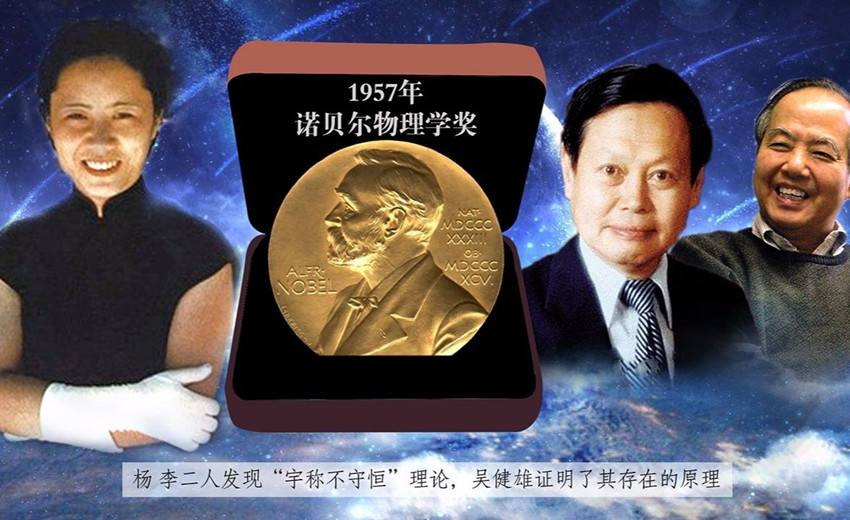
\includegraphics[width=0.8\textwidth]{figs/2021-12-18-00-23-17.png} \\
\end{frame} 





